\chapter{Foundations}
\label{chap:2}

Our reinforcement problem is described by a black-box function that only provides discrete values at the evaluation points. Bayesian optimization is well suited to solve such an optimization problem that does not supply any derivatives.

\section{Bayesian optimization}

% \begin{wrapfigure}{R}{0.5\textwidth}
%     \centering
%     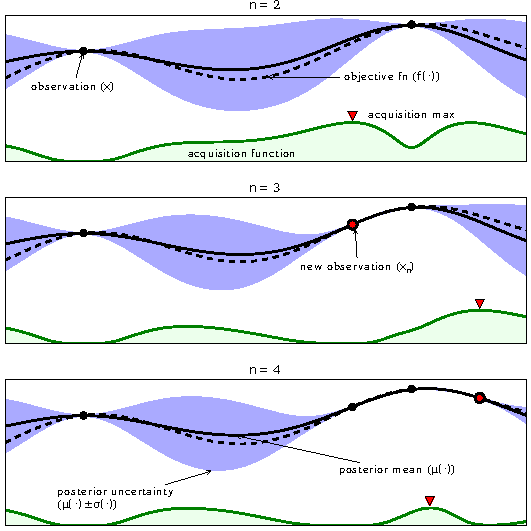
\includegraphics[width=0.45\textwidth]{/home/sebastian/Documents/bscThesis/img/boAcq_brochu2010.pdf}
%     \caption{Visualization of the change in the Gaussian process model and the resulting acquisition function. With every Bayesian optimization iteration step a new observation point at the maximum of the acquisition function is added to the training data. This new observation and its evaluation update the Gaussian process model. Thus the model becomes increasingly accurate in the vicinity of each observation. \cite{brochu2010tutorial} \label{fig:acqBO}}
% \end{wrapfigure}

To find the maximum point of a costly black box target function, we use Bayesian optimization \cite{brochu2010tutorial,shahriari2016taking,lizotte2008practical}. It makes the search process more efficient by incorporating a Gaussian process model to anticipate the objective function's behaviour. This model, containing estimates of the function's returns depending on points, is used by a so called acquisition function to guide the exploration for promising new points. Each selected point is evaluated by the objective function and the results are included in the Gaussian process model. Optimally these steps are repeated until found function values converge at the maximum possible function value. In reality (algorithm \ref{alg:boGlob}) we iterate over $n_{BO}$ steps and analyse the results. The change of the Gaussian process model affecting the acquisition function during Bayesian optimization iterations is illustrated in figure \ref{fig:acqBO}.\\

\begin{algorithm}
    \caption{Global Bayesian optimization\label{alg:boGlob}}
    \SetKwInOut{Input}{input}\SetKwInOut{Output}{output}
    \Input{$X$ = $n_s$ uniformly random samples from the search space\\$n_{BO}$ = number of Bayesian optimization iterations\\set hyper parameters to 1}
    \Output{$\mathbf{x}_{n_{BO} + n_s}$}
    \BlankLine

    $\mathbf{y}$ = evaluations of the objective at the training points $X$\\
    \For{$n$ = $n_s$ \KwTo $n_{BO} + n_s$}{
        optimize hyper parameters (optional)\\
        prepare a Gaussian process model depending on $X$, $\mathbf{y}$ and hyper parameters\\
        $\mathbf{x}_{n+1}$ = point at the optimum of the acquisition function that uses the Gaussian process model\\
        $\mathbf{y}_{n+1}$ = evaluation of the objective at the point $\mathbf{x}_{n+1}$\\
        $X = \{X, \mathbf{x}_{n+1}\}$\\
        $y = \{y, \mathbf{y}_{n+1}\}$\\
    }
\end{algorithm}

The optimization of hyper parameters is optional and depends on the Gaussian process kernel as mentioned in chapter \ref{chap:6}. Also the noise level parameter $\sigma_n$ \eqref{eq:kNoise} is not considered as hyper parameter in this context.

\begin{figure}[h]
    \centering
    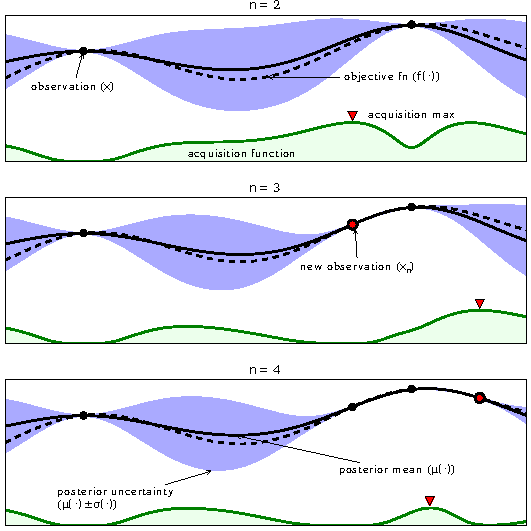
\includegraphics{/home/sebastian/Documents/bscThesis/img/boAcq_brochu2010.pdf}
    \caption{Visualization of the change in the Gaussian process model and the resulting acquisition function \cite{brochu2010tutorial}. The x-axis contains the search space over a one-dimensional example problem. With every Bayesian optimization iteration step a new observation point at the maximum of the acquisition function is added to the training data. This new observation and its evaluation update the Gaussian process model. Thus the model becomes increasingly accurate in the vicinity of each observation. The number of observations is equal the number of iterations and is denoted by $n$. \label{fig:acqBO}}
\end{figure}

\subsection{Gaussian Process Regression}
The Gaussian process finds a prior distribution over the possible functions that are consistent with the training data. From the regression we get a posterior mean and variance, which describe our model of the objective function \cite{rasmussen2006gaussian}. The mean represents a prediction of the true objective at a given point and the variance represents the uncertainty at that point. The more training points our model incorporates the smaller the variance, and the more precise the predictions, in the proximity around training points.\\
In real world applications we always have some noise in the objective observations. Therefore a Gaussian distributed error term,

$$\epsilon \sim \mathcal{N}(0,\sigma_n^2),$$

with zero mean and $\sigma_n^2$ variance is added to the function value. Ergo the observed target

$$\mathbf{y} = f(\mathbf{x}) + \epsilon$$

regards this noise \cite{brochu2010tutorial,shahriari2016taking,lizotte2008practical,rasmussen2006gaussian}. The knowledge our training data provides is represented by the covariance matrix $K(X,X)$. With the matrix of test points $X_*$ we get the joint distribution of the target values and the estimated function values at the test locations \cite{rasmussen2006gaussian}:

$$\left[ \begin{array}{c} \mathbf{y} \\ f_* \end{array} \right] \sim \mathcal{N} \left(0, \begin{bmatrix} K(X,X)+\sigma_n^2 I & K(X,X_*) \\ K(X_*,X) & K(X_*,X_*) \end{bmatrix} \right).$$

For further simplification we define $K = K(X,X)$, $K_* = K(X,X_*)$, $K_*^{\top} = K(X,X_*)^{\top} = K(X_*,X)$, and $K_{**} = K(X_*,X_*)$. Now we can calculate the posterior mean and variance at given test points $X_*$:

\begin{align}
    K_n &= K+\sigma_n^2 I \label{eq:kNoise} \\
    \mathbf{m} &= K_*K_n^{-1}\mathbf{y} \label{eq:meanGauss} \\
    V &= K_{**}-K_*K_n^{-1}K_*^\top \label{eq:wholeVar} \\
    \mathbf{v} &= \mathrm{diag}(V) \label{eq:vectorVar} \\
    \mathbf{s}_\mathrm{dv} &= \sqrt{\mathbf{v}}. \label{eq:gp:stdv}\\ \nonumber
\end{align}

The resulting vectors $\mathbf{m}$ and $\mathbf{v}$ contain the means and variances for all corresponding test points. Also we get the whole covariance matrix $V$.

\subsubsection{Standard kernels}
The similarity between points is measured by the covariance function. The better this covariance function is suited for our objective function the more precise is the resulting model.
We use two standard kernels \cite{rasmussen2006gaussian} to compare them to the trajectory kernel (section \ref{sec:trajKernel}). In those standard kernels the distance metric for two points is given by the Euclidean distance:
$$D(\mathbf{x}_i,\mathbf{x}_j) = (\mathbf{x}_i-\mathbf{x}_j)^\top (\mathbf{x}_i-\mathbf{x}_j).$$

Which we then use in the \textbf{squared exponential kernel},
$$K(\mathbf{x}_i,\mathbf{x}_j,\sigma_f,\sigma_l) = \sigma_{f}^{2}\,\exp\left(-\frac{D(\mathbf{x}_i,\mathbf{x}_j)}{2\sigma_l^2} \right), $$

and the \textbf{Mat\'{e}rn 5/2 kernel},
$$K(\mathbf{x}_i,\mathbf{x}_j,\sigma_f,\sigma_l) = \sigma_{f}^{2}\,\left(1 + \frac{\sqrt{5 D}}{\sigma_l} + \frac{5 D}{3\sigma_l^2} \right) \exp\left(-\frac{\sqrt{5 D}}{\sigma_l} \right),$$

where $\sigma_f$ denote the signal standard deviation and $\sigma_l$ the characteristic length scale. These so called hyper parameters can be tuned by hand or set with hyper parameter optimization.

\subsection{Hyper parameter optimization}

Selecting proper hyper parameters for the Gaussian process regression can reduce the number of objective function evaluations necessary.\\
The likelihood function of the Gaussian process describes the probability of the Gaussian process model being suited for the black box function. To find an optimum for the signal deviation hyper parameter $\sigma_f$ and the length scale hyper parameter $\sigma_l$ we maximize the log likelihood function depending on those parameters \cite{lizotte2008practical}:
\begin{equation} \label{eq:hypOpt}
    \log p(\mathbf{y} = f|X,\sigma_f,\sigma_l) = -\frac{1}{2} \mathbf{y}^\top K_n^{-1} \mathbf{y} -\frac{1}{2} \log |K_n| -\frac{n}{2}\log 2\pi,
\end{equation}

The number of observations is $n$, $X$ is the $d \times n$ dataset of input points and $K_n$ is the covariance matrix for the noisy target $\mathbf{y}$.

\subsection{Acquisition function}
The basis of the Bayesian optimization consists of selecting the next evaluation point in our search space. This point is at the optimum of the acquisition function, which depends on the current Gaussian process model. We choose expected improvement \cite{brochu2010tutorial} during the global Bayesian optimization and in the local optimization (section \ref{sec:localBO}) we use Thompson sampling \cite{akrour2017local}. Both acquisition functions take the mean and the variance generated by the Gaussian process model into account to guide the exploration process. The difficulty lies in avoiding excessive exploration or exploitation. Exploration seeks points with a high variance and exploitation selects points with a high mean instead. The latter one would result in a local optimum whereas too much exploration may not improve at all. An exemplary comparison of acquisition function is shown in figure \ref{fig:acqFcn}.

\begin{figure}[h]
    \centering
    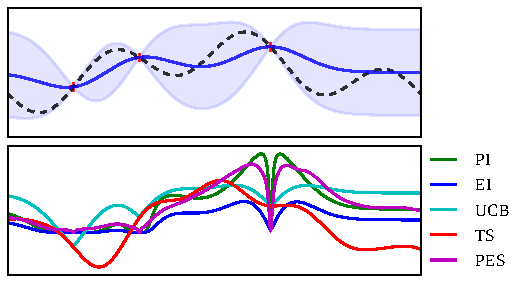
\includegraphics[width=0.70\textwidth]{/home/sebastian/Documents/bscThesis/img/BayesOptLoop_acq_full.pdf}
    \caption{Visualization of Gaussian process posterior values corresponding to different acquisition functions \cite{shahriari2016taking}. The x-axis covers the search space over a one-dimensional example problem. In the upper frame the posterior mean $m$ and double standard deviation $2 \mathbf{s}_{\mathrm{dv}}$ is marked as the blue line with the shaded area. The black dashed line shows the true objective and the red crosses mark already evaluated points. The lower frame compares the plots of the resulting acquisition functions probability of improvement, expected improvement, upper confidence bounds, Thompson sampling and predictive entropy search. The peaks of probability of improvement next to values with high mean illustrates its exploitive behaviour compared to expected improvement, which takes the variance more into account. Thompson sampling is the one with the most explorative peak due to its random nature. \label{fig:acqFcn}}
\end{figure}

\subsubsection{Expected improvement}
To get an expected improvement function value at a test point $\mathbf{x_*}$, we need the mean value $m(\mathbf{x_*})$, and the standard deviation value $\mathbf{s}_{\mathrm{dv}}(\mathbf{x_*}) = \sqrt{v(\mathbf{x_*})}$ from the Gaussian process model. Also we need the maximum of all observations $y_\mathrm{max}$ and a trade-off parameter $\tau$. For the cumulative distribution function, we write $\Phi(.)$ and for the probability density function we write $\phi(.)$. They are both Gaussian with zero mean and unit variance. We adopt the expected improvement function
\[
    \mathrm{EI}(\mathbf{x_*})=
\begin{cases}
    (m(\mathbf{x_*}) - y_\mathrm{max} - \tau)\Phi(\mathrm{z}(\mathbf{x_*}))+\mathbf{s}_{\mathrm{dv}}(\mathbf{x_*})\phi(\mathrm{z}(\mathbf{x_*}))& \text{if } \mathbf{s}_{\mathrm{dv}}(\mathbf{x_*})> 0\\
    0 & \text{if } \mathbf{s}_{\mathrm{dv}}(\mathbf{x_*})= 0
\end{cases}
\]
where
\[
    \mathrm{z}(\mathbf{x_*})=
\begin{cases}
    \frac{(m(\mathbf{x_*}) -y_\mathrm{max} - \tau)}{\mathbf{s}_{\mathrm{dv}}(\mathbf{x_*})} & \text{if } \mathbf{s}_{\mathrm{dv}}(\mathbf{x_*})> 0\\
    0 & \text{if } \mathbf{s}_{\mathrm{dv}}(\mathbf{x_*})= 0
\end{cases}
\]
as suggested in \cite{brochu2010tutorial}. The trade-off parameter $\tau$ can be set to zero or above to gain more exploration. To get the next evaluation point,

$$\mathbf{x}_{n+1} = \arg \max_{\mathbf{x}_*} \mathrm{EI(\mathbf{x}_*)},$$

we optimize the expected improvement function over the whole search space.

\subsubsection{Thompson sampling}
For Thompson sampling acquisition values we sample one function from the Gaussian process posterior \cite{shahriari2016taking},

$$\mathrm{TS}\sim \mathrm{GP}(0,K(X,X_*)),$$

where $X$ is the dataset of already evaluated points, and $X_*$ is a randomly Gaussian distributed set of points with mean and variance given by the local optimizer. These mean and variance represent our current search space.
To draw function values, we need the mean vector $\mathbf{m}$ and the full covariance matrix $V$ from the Gaussian process model. First we take the lower Cholesky decomposite of $V$ such that $L_V L_V^\top = V$. Then we generate a vector $\mathbf{g}$, which consists of independent Gaussian distributed valus with zero mean and unit variance. Finally we get a vector $\mathrm{TS}$ of sampled values:

$$\mathrm{TS}(X_*) = \mathbf{m} + L_V \mathbf{g}.$$

We take the one with the highest value such that,

$$\mathbf{x}_{n+1} = \arg \max_{\mathbf{x}_*} \mathrm{TS}(\mathbf{x}_*),$$

to get the next evaluation point.

\section{Reinforcement learning}

In our reinforcement learning task we want to maximize the cumulative reward stemming from a policy with as few evaluations as feasible. We achieve this maximization by applying Bayesian optimization, treating the cumulative reward as the objective function and policies as points. The objective function evaluation consists of the simulation of a robotic agent.

\subsection{Markov decision process}
We use the Markov decision process model to describe the agent's decisions making \cite{sutton1998reinforcement}. This model consists of a tuple $(S,A,\mathbf{p},\mathbf{r},\gamma)$, holding all states $\mathbf{s}_t \in S$, all actions $a_t \in \mathbf{a}$, all state transitioning probabilities $p_t \in \mathbf{p}$, and all corresponding rewards $r_t \in \mathbf{r}$. The discount factor $\gamma$ is set to 1 because we have a finite horizon Markov decision process where the timing of the reward is irrelevant. Otherwise $\gamma$ would have a value between 0 and 1 to reduce the rewards with increasing time steps. Since the transitioning probabilities and the rewards are unknown, they are accessed through simulation runs of our environment. Assume the agent executing a policy $\mathbf{x}$ for $t_\mathrm{max}$ time steps, producing a trajectory $\xi$, and therefore receiving the final reward

$$\bar{r}(\xi)=\sum_{t=1}^{t_\mathrm{max}} \gamma^t r(\mathbf{s}_{t-1}, \mathbf{a}_{t-1}, \mathbf{s}_{t}),$$

as the sum of all immediate rewards given by a rewarding function $r(\mathbf{s}_{t-1}, \mathbf{a}_{t-1}, \mathbf{s}_{t})$. The explicit probabilities corresponding to actions and state transitionings are also obtained (see \ref{sec:actionselection}) throughout the simulation run.

\subsection{Trajectory kernel}\label{sec:trajKernel}
Standard kernels like the squared exponential kernel, relate policies by measuring the difference between policy parameter values. Therefore policies with similar behaviour but different parameters are not compared adequately. The behaviour based trajectory kernel fixes this, by relating policies to their resulting behaviour \cite{wilson2014using}. This makes our policy search more efficient, since we avoid redundant search of different policies with similar behaviour.

\subsubsection{Behaviour based measurement}

For relating policies to their resulting behaviour we use the Markov decision process transitioning probabilities. We formulate the conditional probability of observing trajectory $\xi$ given policy $\mathbf{x}$ as proposed in \cite{wilson2014using}:

$$p(\xi|\mathbf{x}) = p_{0}(\mathbf{s}_{0}) \prod_{t=1}^{t_\mathrm{max}} p(\mathbf{s}_{t}|\mathbf{s}_{t-1}, \mathbf{a}_{t-1}) p_{\pi}(\mathbf{a}_{t-1}|\mathbf{s}_{t-1}, \mathbf{x}).$$

Trajectory $\xi=(\mathbf{s}_{0},\mathbf{a}_{0}, ..., \mathbf{s}_{t_\mathrm{max}-1}, \mathbf{a}_{t_\mathrm{max}-1}, \mathbf{s}_{t_\mathrm{max}})$ contains the sequence of state, action tuples and policy $\mathbf{x}$ a set of $d$ parameters. The probability of starting in the initial state $\mathbf{s}_{0}$ is denoted by $p_{0}(\mathbf{s}_{0})$, and $p(\mathbf{s}_{t}|\mathbf{s}_{t-1}, \mathbf{a}_{t-1})$ is the probability of transitioning from state $\mathbf{s}_{t-1}$ to $\mathbf{s}_{t}$ when action $\mathbf{a}_{t-1}$ is executed. The stochastic mapping $p_{\pi}(\mathbf{a}_{t-1}|\mathbf{s}_{t-1},\mathbf{x})$ is the probability for selecting the action $\mathbf{a}_{t-1}$ when in state $\mathbf{s}_{t-1}$ and executing the parametric policy $\mathbf{x}$.

\subsubsection{Distance metric}
To examine the difference between two policies $\mathbf{x}_{ i }$ and $\mathbf{x}_{ j }$ the discrete Kullback-Leibler divergence

$$\mathrm {KL}(p(\xi|\mathbf{x}_{ i })||p(\xi|\mathbf{x}_{ j })) = \sum _{\xi in \xi_i}p(\xi|\mathbf{x}_{ i })\,\log {\frac {p(\xi|\mathbf{x}_{ i })}{p(\xi|\mathbf{x}_{ j })}}.$$

is applied to the policy-trajectory mapping probabilities $p(\xi|\mathbf{x}_{ i })$ and $p(\xi|\mathbf{x}_{ j })$ \cite{wilson2014using}. The Kullback-Leibler divergence measures how the two distributions diverge from another.\\

In general $\mathrm {KL}(p(\xi|\mathbf{x}_{ i })||p(\xi|\mathbf{x}_{ j }))$ is not equal to $\mathrm {KL}(p(\xi|\mathbf{x}_{ j })||p(\xi|\mathbf{x}_{ i }))$. But we need a symmetric distance measure. So we sum up the two divergences

$$D(\mathbf{x}_{ i }, \mathbf{x}_{ j }) = \mathrm {KL}(p(\xi|\mathbf{x}_{ i })||p(\xi|\mathbf{x}_{ j })) + \mathrm {KL}(p(\xi|\mathbf{x}_{ j })||p(\xi|\mathbf{x}_{ i })),$$

to achieve that $D(\mathbf{x}_{ i }, \mathbf{x}_{ j }) = D(\mathbf{x}_{ j }, \mathbf{x}_{ i })$. An additional requirement for the kernel is the resulting matrix to be positive semi-definite and scalable\cite{wilson2014using}. Therefore we exponentiate the negative of our distance matrix $D$. We also apply the hyper parameters $\sigma_f^2$ to compensate for the signal variance and $\sigma_l^2$ to adjust for signal length scale. This gives us the covariance function

\begin{equation} \label{eq:trajKernel}
K(\mathbf{x}_{ i },\mathbf{x}_{ j },\sigma_f,\sigma_l) = \sigma_f^2 \exp\left(-\frac{D(\mathbf{x}_i,\mathbf{x}_j)}{2\sigma_l^2} \right).
\end{equation}

In addition to the distance metric proposed by \cite{wilson2014using} we included the signal variance hyper parameter $\sigma_f^2$.

\subsubsection{Estimation of Trajectory Kernel Values}
To reduce the computational effort an estimation of kernel values is applied. The approximation with the Monte-Carlo estimate

\begin{equation} \label{eq:tk:mc}
    \hat{D}(\mathbf{x}_{ i }, \mathbf{x}_{ j }) = \sum _{\xi \in \xi_i} \log\left( \frac{p(\xi|\mathbf{x}_{ i })}{p(\xi|\mathbf{x}_{ j })} \right) + \sum _{\xi \in \xi_j} \log\left( \frac{p(\xi|\mathbf{x}_{ j })}{p(\xi|\mathbf{x}_{ i })} \right)
\end{equation}

is sufficient to measure the divergences between policies with already sampled trajectories \cite{wilson2014using}. $\xi_i$ is the set of trajectories generated by policy $\mathbf{x}_i$. For our Gaussian process regression, we also need a distance measure between a policy with known trajectories and new policies with unknown trajectories. Since there is no closed form solution to this we use the importance sampled divergence

$$\hat{D}(\mathbf{x}_\mathrm{ * }, \mathbf{x}_{ j }) = \sum _{\xi \in \xi_j} \left[\frac{p(\xi|\mathbf{x}_\mathrm{ * })}{p(\xi|\mathbf{x}_{ j })}\,\log\left(\frac{p(\xi|\mathbf{x}_\mathrm{ * })}{p(\xi|\mathbf{x}_{j})}\right)+\log\left(\frac{p(\xi|\mathbf{x}_{ j })}{p(\xi|\mathbf{x}_\mathrm{ * })}\right)\right] $$

to estimate the divergence between the new policy $\mathbf{x}_\mathrm{ * }$ and the policy $\mathbf{x}_j$ with already sampled trajectories $\xi_j$ \cite{wilson2014using}.

Since we only have a ratio of transitioning probabilities present in our trajectory kernel we can reduce the logarithmic term to:

\begin{align*}
    \log\left(\frac{p(\xi|\mathbf{x}_i)}{p(\xi|\mathbf{x}_j)}\right)
    &= \log\left(\frac{p_{0}(\mathbf{s}_{0}) \prod_{t=1}^{t_\mathrm{max}} p_s(\mathbf{s}_{t}|\mathbf{s}_{t-1},\mathbf{a}_{t-1}) p_{\pi}(\mathbf{a}_{t-1}|\mathbf{s}_{t-1},\mathbf{x}_i)}{p_{0}(\mathbf{s}_{0}) \prod_{t=1}^{t_\mathrm{max}} p_s(\mathbf{s}_{t}|\mathbf{s}_{t-1},\mathbf{a}_{t-1}) p_{\pi}(\mathbf{a}_{t-1}|\mathbf{s}_{t-1},\mathbf{x}_j)}\right)\\
    &= \log\left(\prod_{t=1}^{t_\mathrm{max}}\frac{ p_{\pi}(\mathbf{a}_{t-1}|\mathbf{s}_{t-1},\mathbf{x}_i)}{p_{\pi}(\mathbf{a}_{t-1}|\mathbf{s}_{t-1},\mathbf{x}_j)}\right)\\
    &= \sum_{t=1}^{t_\mathrm{max}} \log \left(\frac{p_{\pi}(\mathbf{a}_{t-1}|\mathbf{s}_{t-1},\mathbf{x}_i)}{p_{\pi}(\mathbf{a}_{t-1}|\mathbf{s}_{t-1},\mathbf{x}_j)}\right).
\end{align*}

Summing up the logarithms of the probability ratios in the end is also numerically more stable than computing the logarithm of the products.
